\documentclass[12pt,letterpaper]{article}
\usepackage{fullpage}
\usepackage[top=2cm, bottom=4cm, left=2.5cm, right=2.5cm]{geometry}
\usepackage{amsmath,amsthm,amsfonts,amssymb,amscd}
\usepackage{lastpage}
\usepackage{enumerate}
\usepackage{fancyhdr}
\usepackage{mathrsfs}
\usepackage{xcolor}
\usepackage{graphicx}
\usepackage{listings}
\usepackage{hyperref}
\usepackage{float}

\hypersetup{%
  colorlinks=true,
  linkcolor=blue,
  linkbordercolor={0 0 1}
}
 
\renewcommand\lstlistingname{Algorithm}
\renewcommand\lstlistlistingname{Algorithms}
\def\lstlistingautorefname{Alg.}

\lstdefinestyle{Python}{
    language        = Python,
    frame           = lines, 
    basicstyle      = \footnotesize,
    keywordstyle    = \color{blue},
    stringstyle     = \color{green},
    commentstyle    = \color{red}\ttfamily
}

\setlength{\parindent}{0.0in}
\setlength{\parskip}{0.05in}
\begin{document}
Sunny Lee
\begin{enumerate}
    \item Using the fixed point method, we find the function 
    $g(x) = \pi + \frac{1}{2}\sin{\frac{x}{2}}$ equals $x$ at the point $(3.627, 3.627)$\\
    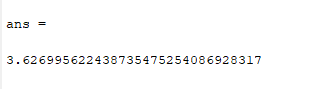
\includegraphics{number1.png}. \\
    Looking at the graph of $g\prime(x)$, we find the maximum value of $g\prime(x)$
    are at the endpoints. So taking $g\prime(x)$ at $x = 0$, we find that: 
    \begin{gather*}
      |g\prime(x)| = |\frac{\cos{\frac{x}{2}}}{4}| = \frac{\cos(0)}{4} = \frac{1}{4}\\
      |g\prime(x)| \leq \frac{1}{4} = k
    \end{gather*}
    To find the number of iterations theoretically required to reach an intersection 
    with an accuracy of $10^{-2}$: 
    \begin{gather*}
      10^{-2} \leq \frac{k^n}{1-k} |p_1 - p_0|
    \end{gather*}
    Using $p_0 = \pi$ and $k = .25$: 
    \begin{gather*}
      10^{-2} \leq \frac{.25^n}{1-.25} |(\pi + .5) - \pi| = \frac{.25^n}{.75} |.5|\\
      \ln{\frac{ 10^{-2} \cdot .75 }{.5}} \leq n\ln{.25}\\
      \frac{\ln{\frac{ 10^{-2} \cdot .75 }{.5}}}{\ln{.25}} \leq n\\
      3.0294 \leq n
    \end{gather*}
    So, we expect to have  4 iterations to reach an approximation with an error $10^{-2}$.
    Starting the fixed point iteration at $x = \pi$, we find it takes 3 iterations 
    to reach an approximation within $10^{-2}$, which fits closely with our 
    theoretical number of iterations. 
    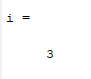
\includegraphics{number1error.png}\\

    \item 
    \begin{enumerate}
      \item 
      Given the equation $2 + \sin(x) - x = 0$, we can add $x$ to the rhs to get 
      $2+\sin(x) = x$ so we obtain $g(x) = 2+\sin(x)$. Looking at the graph of 
      $g'(x)$: 
      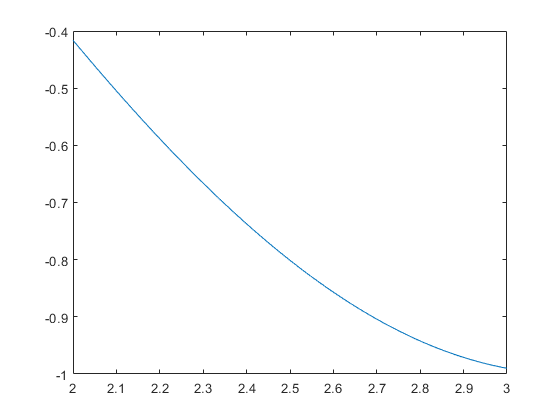
\includegraphics{number2a.png}\\
      $g'(x)$ is a strictly decreasing function on this interval, so we take 
      $g'(x)$ at $x = 3$. 
      \begin{gather*}
        |g'(3)| = |\cos(3)| \approx .99 = k
      \end{gather*}
      Taking $k = .99$: 
      \begin{gather*}
        \frac{10^{-5}(1-.99)}{g(2.5) - 2.5} \leq .99^n\\
        1373.0998 \leq n
      \end{gather*}
      So it would take about 1374 iterations to reach an accuracy within $10^{-5}$. 
      Using MATLAB to estimate the root: \\
      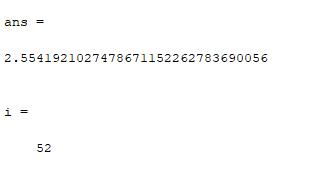
\includegraphics{number2aa.png}\\
      We see it only takes 52 iterations to reach an accuracy of $10^{-5}$.

      \item 
      Given $3x^2 - e^x = 0$, we can reformulate the function as $x = \ln(3x^2)$ using 
      the interval $[3, 4]$, 
      and looking at the graph, we see it is a strictly increasing function. 
      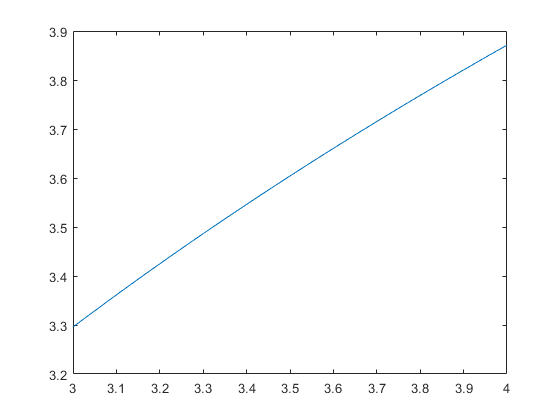
\includegraphics{number2bgraph.png}\\
      Since it is strictly increasing, we only have to check the end points $x = 3,4$ 
      as our $k$ value.\\
      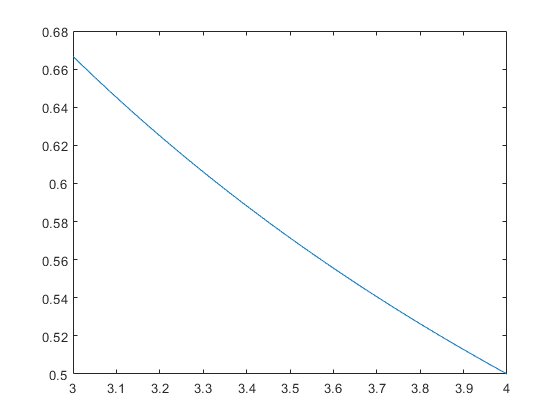
\includegraphics{number2bgraphb.png} \\
      From our graph of the derivatve, we find that $g'(x)$ attains a maximum value 
      at $x = 3$, so our $k$ value is $\frac{2}{3}$. To obtain a number of iterations: 
      \begin{gather*}
        \frac{10^{-5}(1-\frac{2}{3})}{g(3.7) - 3.7} \leq (\frac{2}{3})^n\\
        20.79 \leq n
      \end{gather*}
      So it would take around 21 iterations to get an accuracy of $10^{-5}$. \\
      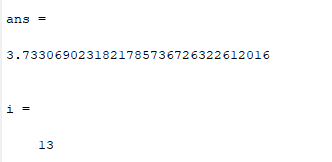
\includegraphics{number2b.png}\\
      We see it only takes 13 iterations to reach an accuracy of $10^{-5}$.
    \end{enumerate}

    \item 
    By reformulating the function to use with our fixed point method: 
    \begin{gather*}
      \ln(\frac{s_0k^2}{m^2g} + \frac{k}{m}t + 1) \cdot -\frac{m}{k} = t
    \end{gather*}
    \\
    Graphing the function $y = x$ and the reformulation: \\
    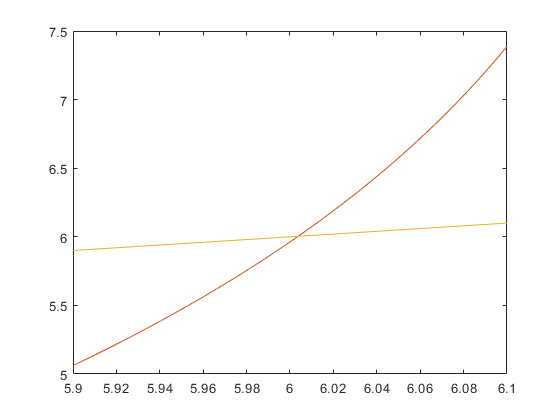
\includegraphics{number3.png}\\
    We see they intersect at around $(6, 6)$ , so taking our initial $p_0 = 6$ 
    we find that the fixed point method converges to around $6.006$: \\
    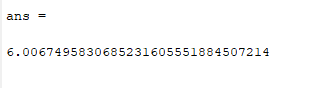
\includegraphics{number3a.png}\\
    
\end{enumerate}

\end{document}